% Generated by experiments/icpc/make_result_figs.py from committed results. Do not edit by hand.
\documentclass[border=2pt]{standalone}
\usepackage[T1]{fontenc}\usepackage{newtxtext,newtxmath}\usepackage[varqu,scaled=0.95]{zi4}
\usepackage{pgfplots}\pgfplotsset{compat=1.18}
\definecolor{cblue}{HTML}{0072B2}\definecolor{cver}{HTML}{D55E00}\definecolor{cora}{HTML}{E69F00}
\definecolor{cgreen}{HTML}{009E73}\definecolor{cgrey}{HTML}{999999}\definecolor{csky}{HTML}{56B4E9}\definecolor{cpurple}{HTML}{7E57C2}
\pgfplotsset{every axis/.append style={font=\footnotesize, tick label style={font=\scriptsize},
  label style={font=\footnotesize}, legend style={font=\scriptsize, draw=none, fill=none},
  axis lines*=left, ymajorgrids, grid style={black!8}}}
\begin{document}
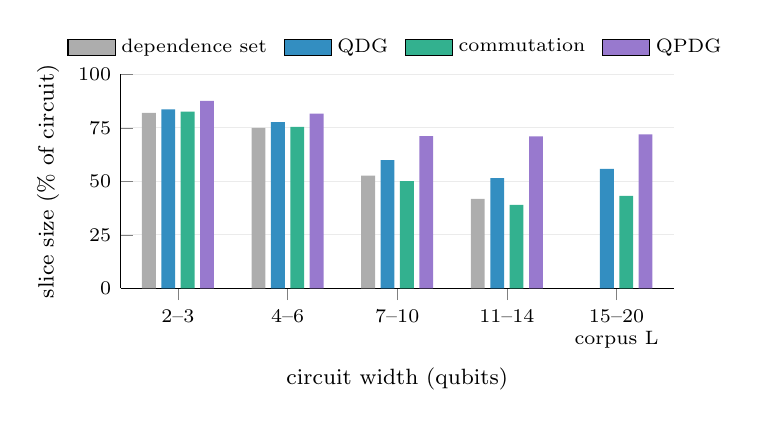
\begin{tikzpicture}\begin{axis}[ybar, bar width=5pt, width=8.6cm, height=4.3cm, ymin=0, ymax=100,
 ytick={0,25,50,75,100}, ylabel={slice size (\% of circuit)}, xlabel={circuit width (qubits)},
 symbolic x coords={a,b,c,d,e}, xtick={a,b,c,d,e}, xticklabels={2--3,4--6,7--10,11--14,{15--20\\corpus L}},
 xticklabel style={align=center}, enlarge x limits=0.13,
 legend style={at={(0.5,1.03)}, anchor=south, legend columns=4, /tikz/every even column/.append style={column sep=4pt}}, area legend]
\addplot[fill=cgrey!80, draw=none] coordinates {(a,82.0) (b,75.0) (c,52.7) (d,41.8)};
\addplot[fill=cblue!80, draw=none] coordinates {(a,83.6) (b,77.7) (c,59.9) (d,51.5) (e,55.8)};
\addplot[fill=cgreen!80, draw=none] coordinates {(a,82.6) (b,75.5) (c,50.1) (d,39.0) (e,43.2)};
\addplot[fill=cpurple!80, draw=none] coordinates {(a,87.6) (b,81.7) (c,71.2) (d,71.0) (e,72.0)};
\legend{{dependence set},{QDG},{commutation},{QPDG}}
\end{axis}\end{tikzpicture}
\end{document}
